\documentclass[a4paper]{article}

\usepackage[
backend=biber,
style=alphabetic,
]{biblatex}
\addbibresource{references.bib}
\usepackage{hyperref}

\usepackage{graphicx}
\graphicspath{ {./images/} }

\usepackage{listings}

\title{Project Proposal}
\author{Matthew Hammond\\2191335\\Vincent Rahli}
\date{October 2023}

\begin{document}

\maketitle

\section{Introduction}
Functional programming is an increasingly popular paradigm, from it's inception in 1950 with Lisp, it was identified as an important paradigm for creating robust, testable, and scalable code \cite{10.1093/comjnl/32.2.98}. The 2015 review of Hughes' article by Hu et al. \cite{10.1093/nsr/nwv042} highlighted the explosion of functional features, especially higher order functions, in modern languages such as C\#, C++, and Java, as well as how further research has led to improved performance of lazy evaluation.

It's no surprise that this has also led to a rise in functional programming within both online and university courses. \cite{warwickFP, kentFP, birminghamFP, courseraFP} Typically these are taught after imperative programming, as functional is seen as having harder concepts, some of which are summarised below.
\subsection{Pure vs Impure}
A pure function is a function with no side effects. A side effect can be anything from reading and writing external state, to non-determinism. A pure function only depends on its inputs, and is unaffected by anything else, which means calling it with the same arguments always result in the same return value.

Pure functions are easier to test, as only their inputs must be supplied and their outputs recorded, but impure functions may require construction of a specific global state before running, and checking the global state after running.
\begin{lstlisting}[language=python, caption=A pure and impure function.]
  def pure(x, y):
      return x + y

  def impure():
      return input(">>")
\end{lstlisting}
Calling the impure function can return many different inputs, and affect the outcomes of other running programs.
This adds additional complexity. How can we read and write files, or take user input while keeping our program pure?\\
The answer is, we can't. IO is inherently impure unless you extend your functions to take the entire world, as described by Peyton Jones \cite{peytonjones2001tackling}.
\begin{lstlisting}[language=haskell]
  pureInput :: World -> (String, World)
  pureOutput :: (String, World) -> World
\end{lstlisting}
\subsection{Lazy vs Eager}
In a language with lazy evaluation, impure functions are especially dangerous. The order of operations could be completely different. Peyton Jones goes on to describe the situation of a list of calls to a Haskell's "printChar" function.
\begin{lstlisting}[language=haskell, caption=An example of lazy evaluation gone awry with IO.]
  xs = [printChar 'a', printChar 'b']
\end{lstlisting}
Alone it doesn't have any side effects, and it's even possible to pass it into some methods such as "length" without any output, as "length" does not evaluate each item in the list.
This is the opposite behaviour to an eager evaluated language, where both characters would be printed out when "xs" was allocated. 
\subsection{Functors, Monads, and more, oh my!}
How can we mitigate these issues? It's all well and good to calculate the solution to a problem, but what good is it if we can't see the solution? A pure program with no side effects can perform computation, but not relay that computation to the user in any useful way.

Haskell's solution is to wrap all IO operations return types in an IO Monad, defined as a typeclass. This doesn't purify IO, but informs the programmer than this function is impure, and must be handled in the proper way. (Haskell's "performUnsafeIO", among others, is an exception, which passes the responsibility of safety to the programmer, and can completely break type safety if used improperly)
\begin{lstlisting}[language=haskell, caption=Haskell's Functor and Monad typeclasses.]
  class Functor f where
      fmap :: (a -> b) -> f a -> f b
      (<$) :: a -> f b -> f b
        
  class Applicative m => Monad m where
      (>>=)  :: m a -> (a -> m b) -> m b
      return :: a -> m a
\end{lstlisting}
Functors and Monads enforce that once you enter the realm of IO, it's not possible to safely leave! Using the results of an IO operation require functions to also return IO.
This could be in the form of a single "return" statement, returning a value of type "IO ()", or a more complex result.
The "$>>$=" (pronounced bind) function allows the results of IO functions to be piped into other functions, providing they return an IO type.
The "fmap" function allows functions not designed for IO to take the results of an IO operation. This can be extended in multiple ways to work with multiple argument functions, such as by using the Applicative typeclass, or the "ap" function in Control.Monad.
\begin{lstlisting}[language=haskell, caption=fmap and bind allow IO operations to be used safely]
  reverse :: [a] -> [a]
  getLine :: IO String
  print :: Show s => s -> IO ()

  main :: IO()
  main = fmap reverse getLine >>= print
\end{lstlisting}
\subsection{Visualisers}
There are numerous visualisers, both on and offline with various goals. Some aim to show algorithms and data structures \cite{algo-vis}, and others \cite{cscircles-vis} aim to show step by step execution, showing which variables are in scope and where, and even one which shows execution by rewriting the code in place, allowing it to be run at any intermediate step \cite{visualize-cbn}! Graph based visualisers, such as the SPARTAN visualiser by Waugh Ambridge \cite{SPARTAN}, can effectively show various functional concepts, such as lazy evaluation with thunks and monads.
\section{Challenges}
\subsection{Syntax and Sugar}
Implementing the entirety of the Haskell language is not a feasible goal. Not only is the standard library very large, but many features have a layer of syntactic sugar on top. Examples include lists, do notation, if-then-else statements, switching prefix/infix, e.t.c. 
\begin{lstlisting}[language=haskell, caption=Some of the ways to write a simple list.\cite{syntatic-sugar}]
  listcomma  = [1, 2, 3, 4, 5]
  listinfix  = (1:2:3:4:5:[])
  listprefix = ((:) 1 ((:) 2 ((:) 3 ((:) 4 ((:) 5 [])))))
\end{lstlisting}
To mitigate this, the implementation will focus on single versions of each. Syntactic sugar can be implemented towards the end of development, if there is time to do so, and when it is necessary.
Similarly, it may be useful to restrict some aspects of the current syntax, such as whitespace. Haskell uses significant whitespace in its syntax, e.g lines of let notation must be on the same line, however this is again syntactic sugar for anonymous functions.
\begin{lstlisting}[language=haskell, caption=let notation and the underlying meaning]
    let
      x = 1
      y = 2
    in (x, y)

    (\x -> \y -> (x, y)) 1 2
\end{lstlisting}
An online search for pre-existing Haskell parsers comes up empty, searching "parse Haskell in JavaScript" provides numerous methods and discussions about the opposite problem, parsing JavaScript in Haskell. It is possible to convert Haskell and Haskell-like languages to JavaScript, however the generated JavaScript is not always the most readable, nor is it split into tokens for easy parsing and interpreting.\cite{purescript} A bespoke Haskell parser is not a small task, but by splitting the features as described in the timeline, the parser can be incrementally developed in an extensible way to include extended types and typeclasses.
\subsection{Visualisation}
Visualising execution is also a major part of this milestone, but as seen above is easy to make overwhelming. In Figure \ref{fig:mockup-1} the full visualisation is shown, which only works for small inputs. The shown "add1" function has constant complexity, but a recursive function, a cornerstone of functional programming, would quickly expand with much worse graph complexity.
Figure \ref{fig:mockup-2} shows what visualisation can look like for only the current program state, showing each recursive functional call (and the upcoming function call) as arrows. This can be integrated with step controls to step through the execution, and boxes could be highlighted when recursive calls are made and returned from.
Typically step by step visualisation is used, as it vastly reduces the screen space required to show execution. Especially for imperative languages, where time is also a straightforward component of execution, step by step evaluation 
\begin{figure}[h]
    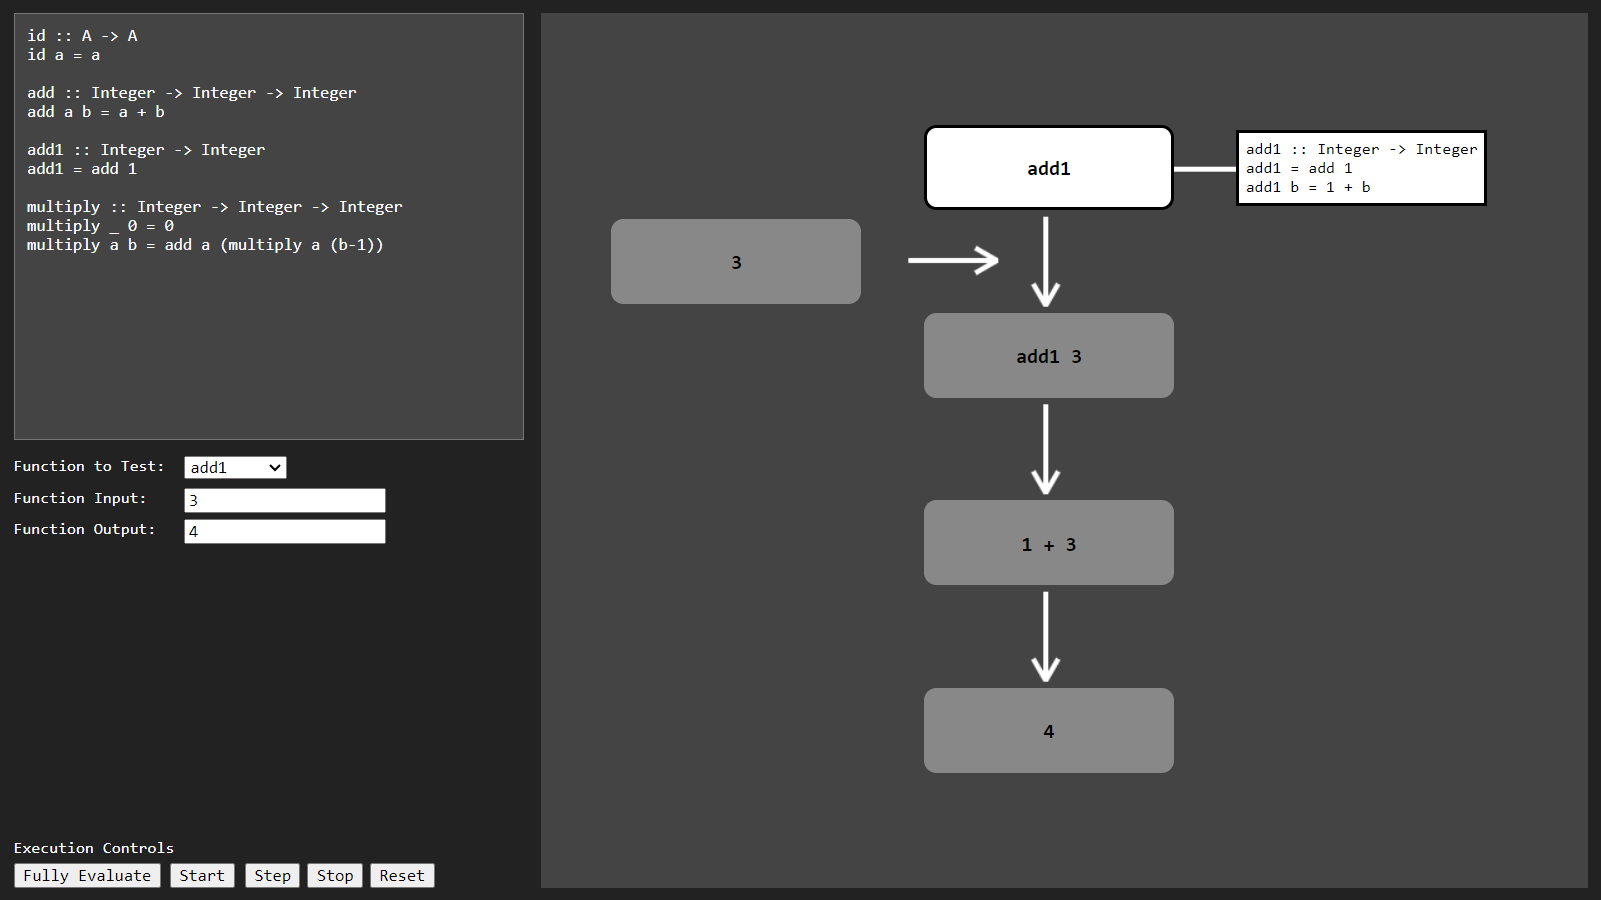
\includegraphics[width=\textwidth]{mockup-1}
    \caption{Full program visualisation}
    \label{fig:mockup-1}
\end{figure}
\begin{figure}[h]
    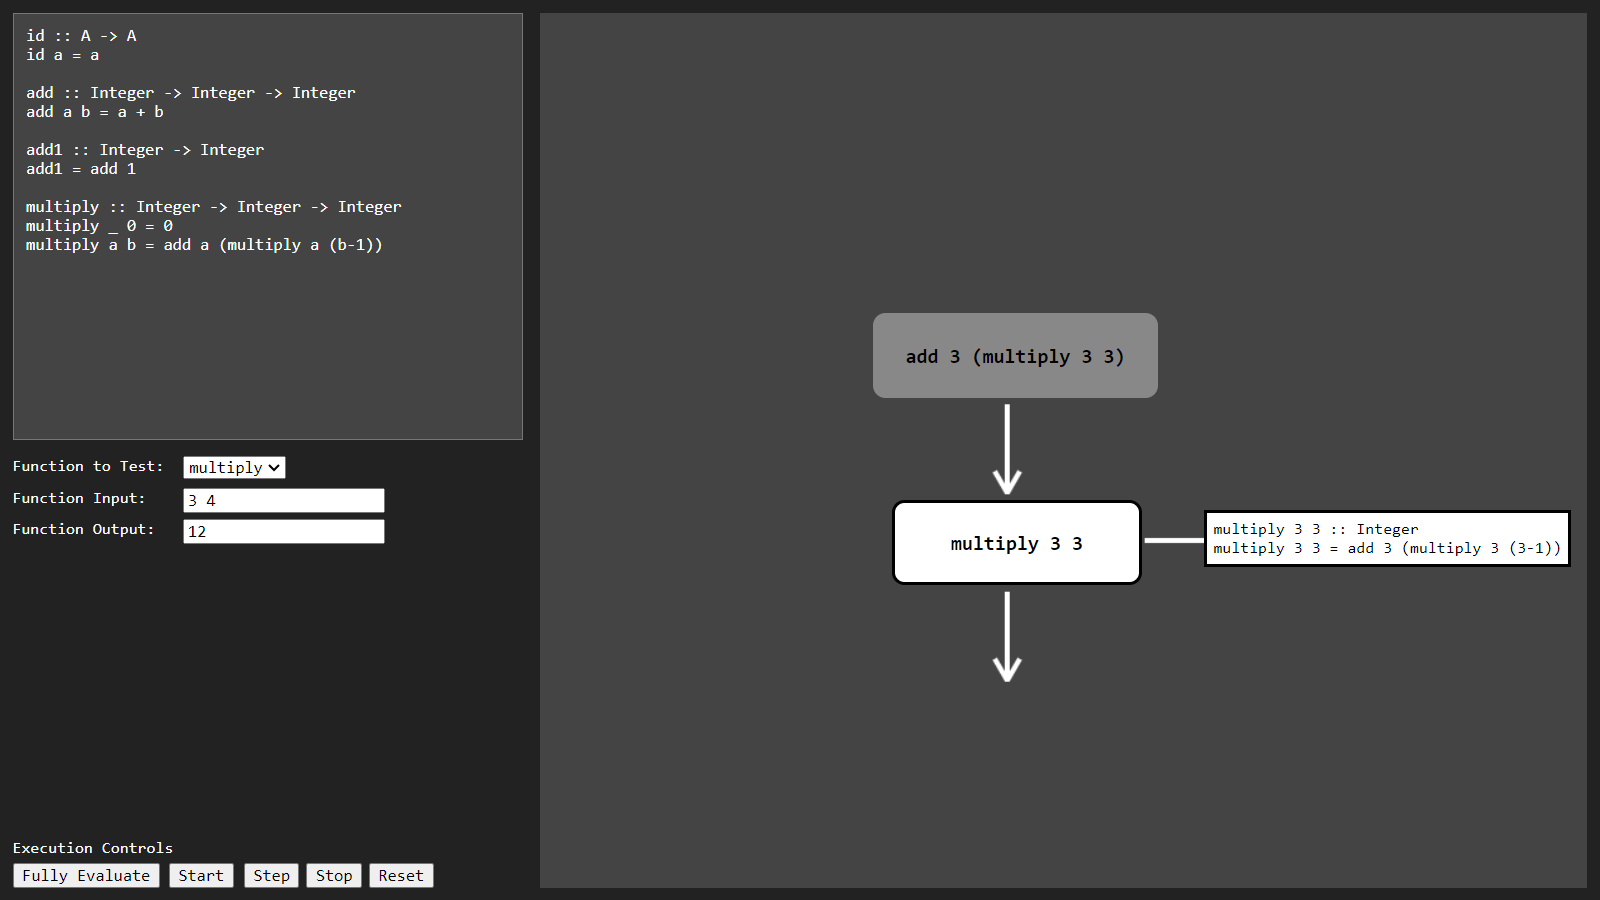
\includegraphics[width=\textwidth]{mockup-2}
    \caption{Visualising only current program state}
    \label{fig:mockup-2}
\end{figure}
\subsection{Type Inference and Type Checking}
Haskell uses polymorphism extensively, functions can be generalised to take any type, which can be restricted using typeclasses.
\begin{lstlisting}[language=haskell, caption=Polymorphism]
    id :: a -> a
    map :: (a -> b) -> [a] -> [b]
    map f (h:t) = f h : map f t
\end{lstlisting}
While the "id" function can take any type, the "map" function cannot. Once a function has been bound to it, the next argument's, and the result's, type are restricted to simply the input and output types of the function.
To ensure that the "map" function is still used correctly, the type of it's second argument must be checked, to ensure "a" is the same "a" as in the first argument.
To mitigate this challenge, all functions will be required to define their type, whereas in Haskell, the type of "map" can be inferred from it's implementation. This will greatly simplify the type checker, as more functions will be explicitly defined.
\section{Milestones}
\subsection{Basic Implementation, Week 1-10}
The core component of a functional languages, are the functions. Which all later features build upon. This includes functions with specific types, as well as generic functions.

Certain functions, such as "+" will be implemented in JavaScript to perform the actual execution, but will still be shown as a normal typed function. This means internally functions could be represented as a pure Haskell function, or as a JavaScript function with the Haskell shown to the user. This will only need to be done for primitive operations, as all others will be able to made out of a composition of primitive operations.

In Figure \ref{fig:mockup-2} the user interface contains an input for the code with some example functions of this milestone, in the top left, the "multiply" function is selected for testing, with the inputs 3 and 4. The execution is shown on the right, with the "multiply 3 3" thunk selected to show extra information, showing that it adds 3 to the result of a recursive call.

Visualisation can be done with a library like Cytoscape.js \cite{cytoscape}. This library has a huge array of customisation options for displaying graphs specifically for visualisation and analysis, and comes with many features that will allow large graphs to be displayed well, such as allowing scaling of the full canvas, as well as moving around individual nodes. It is also available as a minified JavaScript file, which can be easily served on the front end without having to generate the graphs server side.
\subsubsection{Steps}
\begin{itemize}
    \item Implement a user interface, with code, input, and output fields.
    \item Implement parsing of functions, their types, and bodies.
    \item Implement function application, and lazy evaluation.
    \item Display function evaluation in a visual graph-like way using Cytoscape.js.
\end{itemize}
\subsection{Extended Typing, Week 11-14}
\label{extended-typing}
This goal will extend to user defined types, as well as define some of the functions used in Haskell's Prelude module (in which List will be defined as Cons and Nil). The key milestones for this goal will be the "data" and "type" keywords, as they allow for further definition of types in Haskell.
\begin{lstlisting}[language=haskell, caption=Example functions/types of stage 2.]
  data List A = Cons A (List A) | Nil

  map :: (A -> B) -> List A -> List B
  map f Nil         = Nil
  map f (Cons x xs) = Cons (f x) (map f xs)
\end{lstlisting}
\subsubsection{Steps}
\begin{itemize}
    \item Implement parsing of type syntax, "data", "type", and "newtype" keywords, and type variables.
    \item Implement parsing of functions using user-defined types.
    \item Implement a variety of Prelude's built-in types.
    \item Display type construction in a visual graph-like way using Cytoscape.js.
\end{itemize}
\subsection{Typeclasses and Monads, Week 15-18}
Lastly, monads will be implemented. This will require an IO interface, rather than just a raw input into a program. The key milestone for this goal will be the "class" keyword, as that allows for typeclasses, which monads are implemented using.
The key feature of typeclasses is operator overloading. Many instances of the Monad typeclass exists, but the exact function used depends on the data being acted on.
This will also allow for simplification of other functions, by using typeclasses to move the overloaded operators into, for example addition, where each numerical type can define it's own addition, which other functions can then use.

At this point proper IO can be added. The interface can be modified to support both running the program as a whole, through a "main :: IO ()" function, or running a specific function. Console IO could be implemented through HTML's modals, or new input/output boxes specifically for console IO (as running the whole program wouldn't specifically take any inputs, nor output anything). Visually IO could be shown as a simplified form of Peyton Jones' example, taking just the Console, instead of the World as an argument.
\begin{lstlisting}[language=haskell, caption=The Num typeclass. (+) would be implemented in JavaScript.]
  class Num n where
    (+) :: n -> n -> n
    ...

  instance Num Integer where
    a + b = ...
    ...
\end{lstlisting}
\subsubsection{Steps}
\begin{itemize}
    \item Implement parsing of typeclass syntax, "class", "instance", and "where" keywords into the parser.
    \item Implement typeclasses for the defined types in Section \ref{extended-typing} where appropriate in Haskell.
    \item Correct identification and evaluation of the correct operator function.
    \item Implement visually the application of typeclass functions using Cytoscape.js.
\end{itemize}
\printbibliography
\end{document}